\documentclass[10pt]{beamer}

\usetheme{simear}

\title{Implementing QVMP using QROM}
\author{Elton Pinto}
\date{\today}

\usepackage{algorithm}
\usepackage{algpseudocode}
\usepackage[braket, qm]{qcircuit}
\usepackage{subcaption}

\begin{document}

\begin{frame}[plain]
\titlepage
\end{frame}


\begin{frame}{Motivation}
  \begin{itemize}
    \item Grover search: popular quantum search algorithm
    \item Depends on a black-box oracle to perform the search
    \item Offers quadratic speedup over classical linear search with a
      runtime of $O(\sqrt{N})$
  \end{itemize}
  \begin{figure}
    \centering
    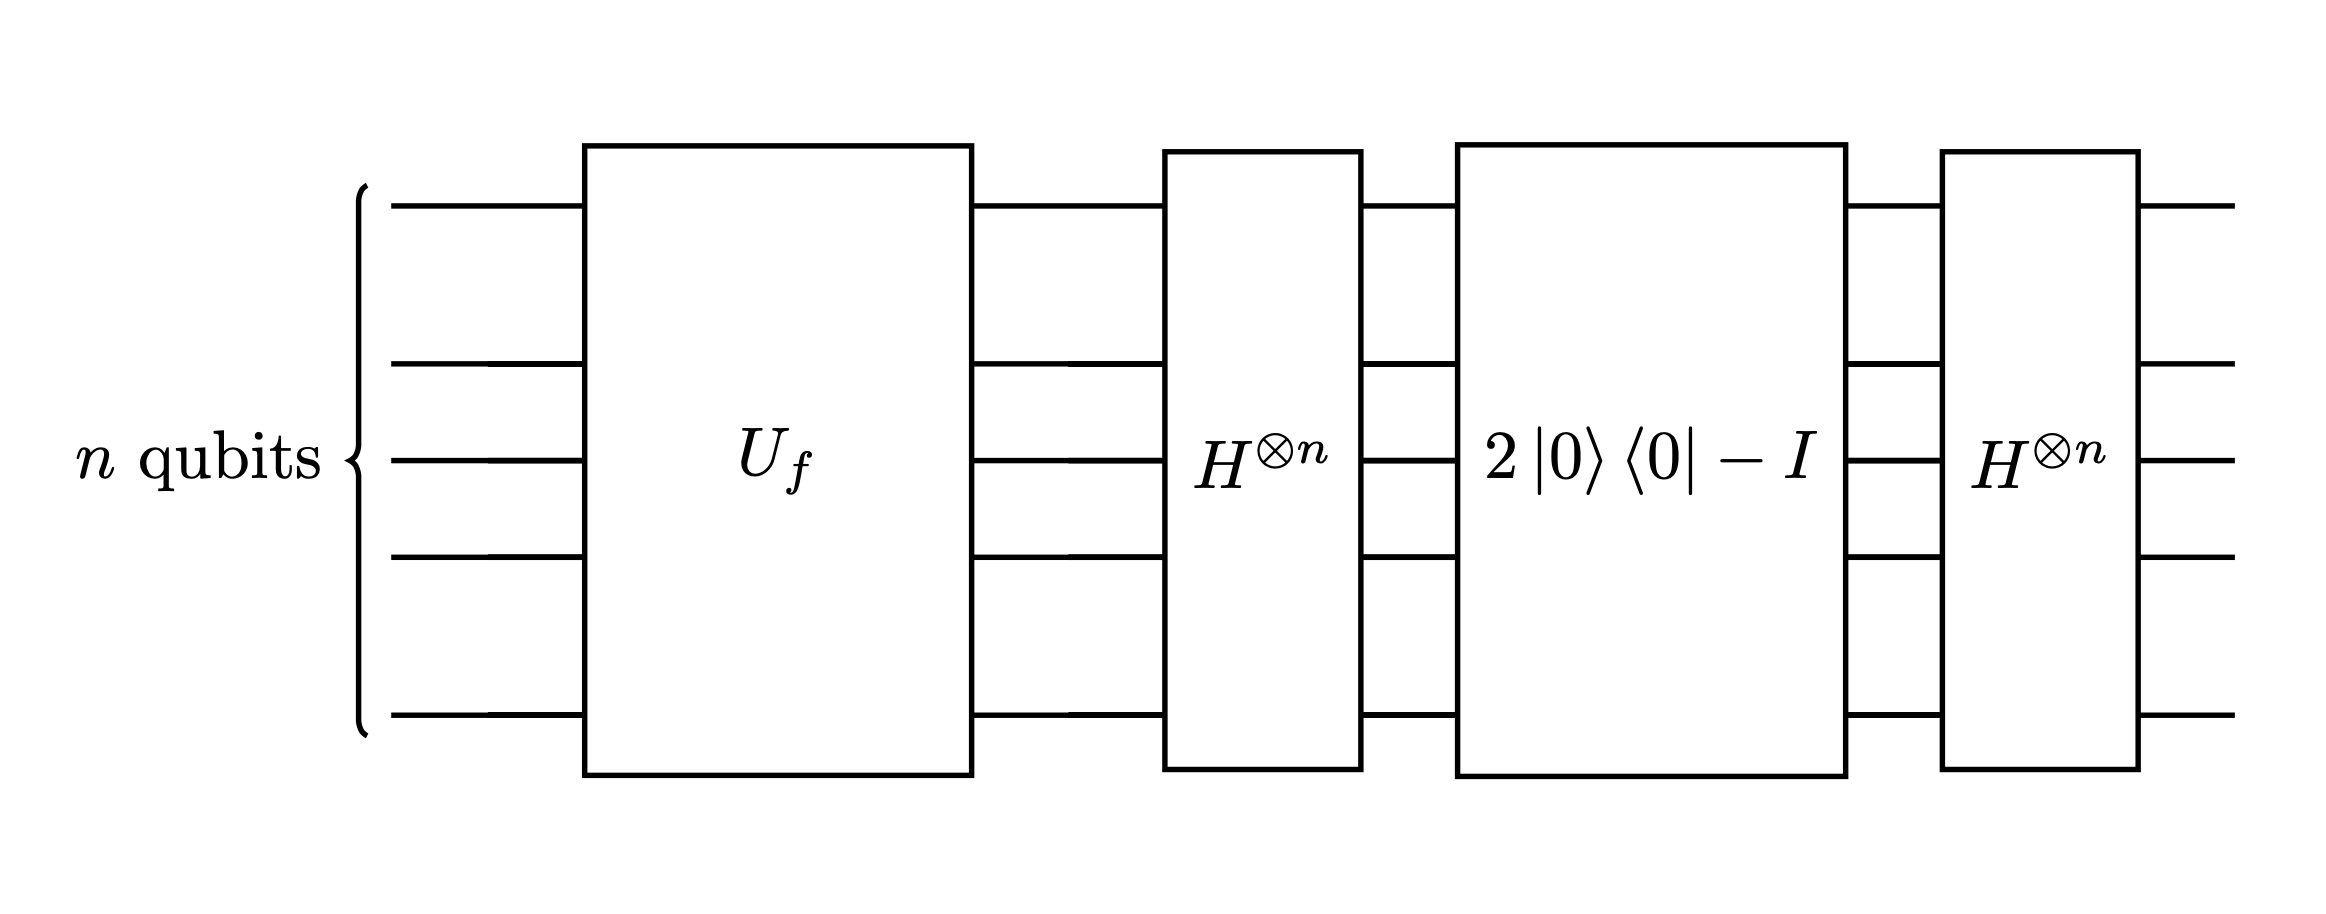
\includegraphics[width=0.7\textwidth]{assets/grover_operator.png}
    \caption{Grover operator circuit}
    \label{fig:grover_operator_circuit}
  \end{figure}
\end{frame}


\begin{frame}{Motivation (contd)}
  \begin{itemize}
    \item Core of Grover search straightforward to implement
    \item {
      Main challenge: encoding the oracle as a quantum circuit
      % \begin{itemize}
      %   \item Debugging oracles is tricky due to non-determinism
      %   \item How to verify correctness?
      % \end{itemize}
    }
    \item {
      QVMP
      \begin{itemize}
        \item Quantum Verification of Matrix Products
        \item Offers quadratic speed-up over classical VMP
        \item Used in HPC applications
        \item Algorithm uses Grover search as a sub-routine
      \end{itemize}
    }
  \end{itemize}

  \begin{alertblock}{Goal}
    Implement QVMP to better understand these challenges, determine feasibility
    of use, and investigate enhancements into oracle encoding
  \end{alertblock}
\end{frame}


\begin{frame}{Main contributions}
  \begin{itemize}
    \item Working implementation of QVMP in Qiskit
    \item Circuit metrics (gate count, circuit depth)
    \item Transpilation and simulation times
  \end{itemize}
\end{frame}


\begin{frame}{QVMP}
  \begin{itemize}
    \item Quantum Verification of Matrix Products
    \item Given $n \times n$ matrices $A$, $B$ and $C$, check if $AB = C$
    \item {
        Two quantum algorithms:
        \begin{itemize}
          \item Grover search based: $O(n^{\frac{7}{4}})$
          \item Quantum random walk based: $O(n^{\frac{5}{3}})$
        \end{itemize}
    }
  \end{itemize}
\end{frame}


% TODO replace this with a picture
\begin{frame}{QVMP Algorithm}
\begin{algorithm}[H]
  \caption{Quantum VMP using Grover Search}
  \label{alg:qvmp_grover}
  \textbf{Input: } $n \times n$ matrices $A, B, C$ \\
  \textbf{Output: } 1 if $AB = C$ and 0 otherwise \\
  \textbf{Procedure: }
  \begin{enumerate}
    \item Partition $B$ and $C$ into sub-matrices of size $n \times \sqrt{n}$
    \item 
      {
        Perform amplitude amplification for $n^{\frac{1}{4}}$ iterations using this subroutine:
        \begin{enumerate}
          \item Pick a random vector $x$ of size $\sqrt{n}$
          \item Classically compute $y = B_ix$ and $z = C_ix$
          \item Using Grover search with $\sqrt{n}$ iterations, find a row of
            index $j$ such that $(Ay \neq z)_j$
        \end{enumerate}
      }
    \item XOR the sub-results
  \end{enumerate}
\end{algorithm}
\end{frame}


\begin{frame}[fragile]{QVMP Implementation}
  \begin{lstlisting}[frame=single,language=Python, numbers=left]
# QVMP oracle described using a classical function

def find_row_mismatch(A, y, z):
  z_prime = A * y
  for j, value in enumerate(z_prime):
    if value != z[j]:
      return j
  return -1
  \end{lstlisting}

  \begin{itemize}
    \item The above snippet is encoded as a quantum circuit and constitutes
      the oracle
    \item QROM is used to efficiently encode the matrix
    \item Out-of-place inner product performs the row-vector multiplication
  \end{itemize}
\end{frame}


\begin{frame}{QROM - Quantum Read-only Memory}
  \begin{itemize}
    \item Encodes an $n \times m$ binary matrix using only $n + \log_2(n)$ qubits
    \item Outputs the value of the $j$th row indexed using address qubits
    \item Can use superposition to extract multiple rows
  \end{itemize}
  \begin{figure}
      \centering
      \scalebox{0.8}{
      \begin{minipage}{\textwidth}
          \begin{equation*}
            A = \begin{bmatrix}%
              0 & 1 & 0 & 1 \\
              1 & 1 & 1 & 0 \\
              1 & 0 & 0 & 1 \\
              1 & 0 & 1 & 0 \\
            \end{bmatrix}
          \end{equation*}
      \end{minipage}
      }
      \begin{subfigure}{\textwidth}
        \centering
        \scalebox{0.8}{
  \begin{minipage}{\textwidth}
    \begin{equation*}
      A = \begin{bmatrix}%
        0 & 1 & 0 & 1 \\
        1 & 1 & 1 & 0 \\
        1 & 0 & 0 & 1 \\
        1 & 0 & 1 & 0 \\
      \end{bmatrix}
    \end{equation*}
  \end{minipage}
}
\begin{subfigure}{\textwidth}
  \centering
  \scalebox{0.8}{
            \Qcircuit @C=1.0em @R=0.2em @!R { \\
  	      \nghost{{addr}_{0} :  } & \lstick{{addr}_{0} :  } & \gate{\mathrm{X}} & \ctrl{1} & \ctrl{1} \barrier[0em]{5} & \qw & \gate{\mathrm{X}} & \ctrl{1} & \ctrl{1} \barrier[0em]{5} & \qw & \qw & \ctrl{1} & \ctrl{1} \barrier[0em]{5} & \qw & \gate{\mathrm{X}} & \ctrl{1} & \ctrl{1} \barrier[0em]{5} & \qw & \qw & \qw\\
  	      \nghost{{addr}_{1} :  } & \lstick{{addr}_{1} :  } & \gate{\mathrm{X}} & \ctrl{2} & \ctrl{4} & \qw & \qw & \ctrl{1} & \ctrl{4} & \qw & \gate{\mathrm{X}} & \ctrl{1} & \ctrl{2} & \qw & \qw & \ctrl{1} & \ctrl{2} & \qw & \qw & \qw\\
  	      \nghost{{data}_{0} :  } & \lstick{{data}_{0} :  } & \qw & \qw & \qw & \qw & \qw & \targ & \qw & \qw & \qw & \targ & \qw & \qw & \qw & \targ & \qw & \qw & \qw & \qw\\
  	      \nghost{{data}_{1} :  } & \lstick{{data}_{1} :  } & \qw & \targ & \qw & \qw & \qw & \qw & \qw & \qw & \qw & \qw & \targ & \qw & \qw & \qw & \targ & \qw & \qw & \qw\\
  	      \nghost{{data}_{2} :  } & \lstick{{data}_{2} :  } & \qw & \qw & \qw & \qw & \qw & \qw & \qw & \qw & \qw & \qw & \qw & \qw & \qw & \qw & \qw & \qw & \qw & \qw\\
  	      \nghost{{data}_{3} :  } & \lstick{{data}_{3} :  } & \qw & \qw & \targ & \qw & \qw & \qw & \targ & \qw & \qw & \qw & \qw & \qw & \qw & \qw & \qw & \qw & \qw & \qw\\
  \\ }}
\end{subfigure}

      \end{subfigure}
      \caption{QROM encoding of a $4 \times 4$ matrix $A$}
      \label{fig:qrom_4x4}
  \end{figure}
\end{frame}


% \begin{frame}{Inner product}
%   \begin{itemize}
%     \item Computes the inner product between two binary vectors using $2n + 1$
%       qubits
%     \item Outputs the result in a separate qubit
%   \end{itemize}
%   \begin{figure}
%     \centering
%     \scalebox{1.0}{
\Qcircuit @C=1.0em @R=0.8em @!R { \\
	 	\nghost{{a}_{0} :  } & \lstick{{a}_{0} :  } & \ctrl{2} & \qw & \qw & \qw\\
	 	\nghost{{a}_{1} :  } & \lstick{{a}_{1} :  } & \qw & \ctrl{2} & \qw & \qw\\
	 	\nghost{{b}_{0} :  } & \lstick{{b}_{0} :  } & \ctrl{2} & \qw & \qw & \qw\\
	 	\nghost{{b}_{1} :  } & \lstick{{b}_{1} :  } & \qw & \ctrl{1} & \qw & \qw\\
	 	\nghost{{out} :  } & \lstick{{out} :  } & \targ & \targ & \qw & \qw\\
\\ }}

%     \caption{Inner product circuit for $2$-D vectors}
%     \label{fig:inner_product}
%   \end{figure}
% \end{frame}


\begin{frame}{QVMP oracle}
  \begin{figure}
    \centering
    \scalebox{0.7}{\scalebox{1.0}{
\Qcircuit @C=1.0em @R=0.2em @!R { \\
	 	\nghost{{address}_{0} :  } & \lstick{{address}_{0} :  } & \gate{\mathrm{H}} \barrier[0em]{10} & \qw & \multigate{10}{\mathrm{db}}_<<<{0} & \qw & \qw & \qw & \multigate{10}{\mathrm{db\_dg}}_<<<{0} \barrier[0em]{10} & \qw & \multigate{1}{\mathrm{diffuser}}_<<<{0} \barrier[0em]{10} & \qw & \meter & \qw & \qw & \qw\\
	 	\nghost{{address}_{1} :  } & \lstick{{address}_{1} :  } & \gate{\mathrm{H}} & \qw & \ghost{\mathrm{db}}_<<<{1} & \qw & \qw & \qw & \ghost{\mathrm{db\_dg}}_<<<{1} & \qw & \ghost{\mathrm{diffuser}}_<<<{1} & \qw & \qw & \meter & \qw & \qw\\
	 	\nghost{{a}_{0} :  } & \lstick{{a}_{0} :  } & \qw & \qw & \ghost{\mathrm{db}}_<<<{2} & \multigate{8}{\mathrm{dot}}_<<<{0} & \qw & \multigate{8}{\mathrm{dot\_dg}}_<<<{0} & \ghost{\mathrm{db\_dg}}_<<<{2} & \qw & \qw & \qw & \qw & \qw & \qw & \qw\\
	 	\nghost{{a}_{1} :  } & \lstick{{a}_{1} :  } & \qw & \qw & \ghost{\mathrm{db}}_<<<{3} & \ghost{\mathrm{dot}}_<<<{1} & \qw & \ghost{\mathrm{dot\_dg}}_<<<{1} & \ghost{\mathrm{db\_dg}}_<<<{3} & \qw & \qw & \qw & \qw & \qw & \qw & \qw\\
	 	\nghost{{a}_{2} :  } & \lstick{{a}_{2} :  } & \qw & \qw & \ghost{\mathrm{db}}_<<<{4} & \ghost{\mathrm{dot}}_<<<{2} & \qw & \ghost{\mathrm{dot\_dg}}_<<<{2} & \ghost{\mathrm{db\_dg}}_<<<{4} & \qw & \qw & \qw & \qw & \qw & \qw & \qw\\
	 	\nghost{{a}_{3} :  } & \lstick{{a}_{3} :  } & \qw & \qw & \ghost{\mathrm{db}}_<<<{5} & \ghost{\mathrm{dot}}_<<<{3} & \qw & \ghost{\mathrm{dot\_dg}}_<<<{3} & \ghost{\mathrm{db\_dg}}_<<<{5} & \qw & \qw & \qw & \qw & \qw & \qw & \qw\\
	 	\nghost{{y}_{0} :  } & \lstick{{y}_{0} :  } & \gate{\mathrm{X}} & \qw & \ghost{\mathrm{db}} & \ghost{\mathrm{dot}}_<<<{4} & \qw & \ghost{\mathrm{dot\_dg}}_<<<{4} & \ghost{\mathrm{db\_dg}} & \qw & \qw & \qw & \qw & \qw & \qw & \qw\\
	 	\nghost{{y}_{1} :  } & \lstick{{y}_{1} :  } & \gate{\mathrm{X}} & \qw & \ghost{\mathrm{db}} & \ghost{\mathrm{dot}}_<<<{5} & \qw & \ghost{\mathrm{dot\_dg}}_<<<{5} & \ghost{\mathrm{db\_dg}} & \qw & \qw & \qw & \qw & \qw & \qw & \qw\\
	 	\nghost{{y}_{2} :  } & \lstick{{y}_{2} :  } & \qw & \qw & \ghost{\mathrm{db}} & \ghost{\mathrm{dot}}_<<<{6} & \qw & \ghost{\mathrm{dot\_dg}}_<<<{6} & \ghost{\mathrm{db\_dg}} & \qw & \qw & \qw & \qw & \qw & \qw & \qw\\
	 	\nghost{{y}_{3} :  } & \lstick{{y}_{3} :  } & \qw & \qw & \ghost{\mathrm{db}} & \ghost{\mathrm{dot}}_<<<{7} & \qw & \ghost{\mathrm{dot\_dg}}_<<<{7} & \ghost{\mathrm{db\_dg}} & \qw & \qw & \qw & \qw & \qw & \qw & \qw\\
	 	\nghost{{z} :  } & \lstick{{z} :  } & \qw & \qw & \ghost{\mathrm{db}}_<<<{6} & \ghost{\mathrm{dot}}_<<<{8} & \gate{\mathrm{Z}} & \ghost{\mathrm{dot\_dg}}_<<<{8} & \ghost{\mathrm{db\_dg}}_<<<{6} & \qw & \qw & \qw & \qw & \qw & \qw & \qw\\
	 	\nghost{\mathrm{{data} :  }} & \lstick{\mathrm{{data} :  }} & \lstick{/_{_{2}}} \cw & \cw & \cw & \cw & \cw & \cw & \cw & \cw & \cw & \cw & \dstick{_{_{\hspace{0.0em}0}}} \cw \ar @{<=} [-11,0] & \dstick{_{_{\hspace{0.0em}1}}} \cw \ar @{<=} [-10,0] & \cw & \cw\\
\\ }}
}
    \caption{QVMP oracle for a $4 \times 4$ matrix $A$ performing one iteration}
    \label{fig:qvmp_oracle}
  \end{figure}
\end{frame}


\begin{frame}{Evaluation}
  \begin{itemize}
    \item Aer simulator provided by Qiskit
    \item Rudimentary noise model
    \item {
        Testbench specs
        \begin{itemize}
          \item AMD EPYC 7502 32-Core Processor, 1498.333 MHz
          \item 128 CPUs
          \item x86\_64 architecture
        \end{itemize}
    }
    \item {
        Simulation methods
        \begin{itemize}
          \item Statevector: Dense statevector simulation, limited by size
          \item Matrix product state (MPS): Tensor-network statevector simulator,
            doesn't model entire quantum state
        \end{itemize}
    }
  \end{itemize}
\end{frame}


\begin{frame}{Evaluation - Functionality}
  \begin{itemize}
    \item \textbf{Input:} $16 \times 16$ matrix $A$ and two vectors $y$ and $z$
      with $(Ay \neq z)_j$ for $j \in \{0, 5, 4\}$
  \end{itemize}
  \begin{figure}
    \centering
    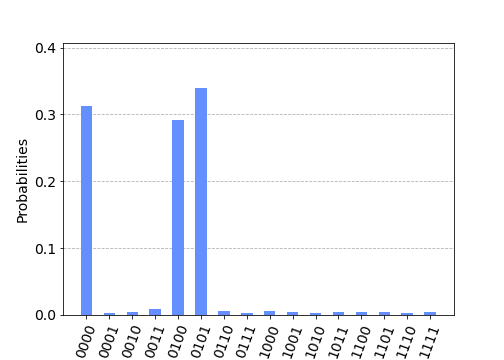
\includegraphics[width=0.7\textwidth]{assets/16x16-simulation.png}
    \caption{Probability of measuring the row-index $j$ after running the QVMP
    oracle}
    \label{fig:qvmp_oracle_sample_execution}
  \end{figure}
\end{frame}


\begin{frame}{Evaluation - Circuit metrics}
  \begin{table}
    \centering
    \begin{subtable}{\textwidth}
      \resizebox{\textwidth}{!}{%
      \begin{tabular}{|c|c||c|c|c|c|c||c|c|c|} 
        \hline
        Dimension & Row mismatches & ccx & cx & x & h & z & Circuit Depth & Qubit count & Gate count \\
        \hline
        (4,4) & 1 & 30 & 1 & 11 & 2 & 1 & 44 & 11 & 49 \\
        (16,8) & 2 & 32 & 10108 & 69 & 284 & 2 & 16993 & 21 & 21494 \\
        (32,4) & 2 & 24 & 42060 & 204 & 461 & 3 & 69510 & 14 & 85299 \\
        (64,8) & 3 & 48 & 300324 & 401 & 1602 & 3 & 497172 & 23 & 604329 \\
        \hline
      \end{tabular}}
      \caption{MPS}
      \label{table:circuit_metrics_mps}
    \end{subtable}

    \begin{subtable}{\textwidth}
      \resizebox{\textwidth}{!}{%
      \begin{tabular}{|c|c||c|c|c|c|c||c|c|c|} 
        \hline
        Dimension & Row mismatches & ccx & cx & x & h & z & Circuit Depth & Qubit count & Gate count \\
        \hline
        (4,4) & 1 & 30 & 1 & 11 & 2 & 1 & 44 & 11 & 49 \\	
        (16,8) & 2 & 32 & 0 & 76 & 4 & 2 & 385 & 21 & 130 \\	
        (32,4) & 2 & 24 & 0 & 208 & 5 & 3 & 684 & 14 & 270 \\
        (64,8) & 3 & 48 & 0 & 405 & 6 & 3 & 2040 & 23 & 498 \\	
        \hline
      \end{tabular}}
      \caption{Statevector}
      \label{table:circuit_metrics_statevector_cpu}
    \end{subtable}
    \caption{Circuit metrics for MPS and statevector simulation methods on
    select dimensions}
    \label{table:circuit_metrics}
  \end{table}
\end{frame}


\begin{frame}{Evaluation - Transpilation vs Simulation}
  \begin{figure}
    \begin{subfigure}{0.48\textwidth}
      \centering
      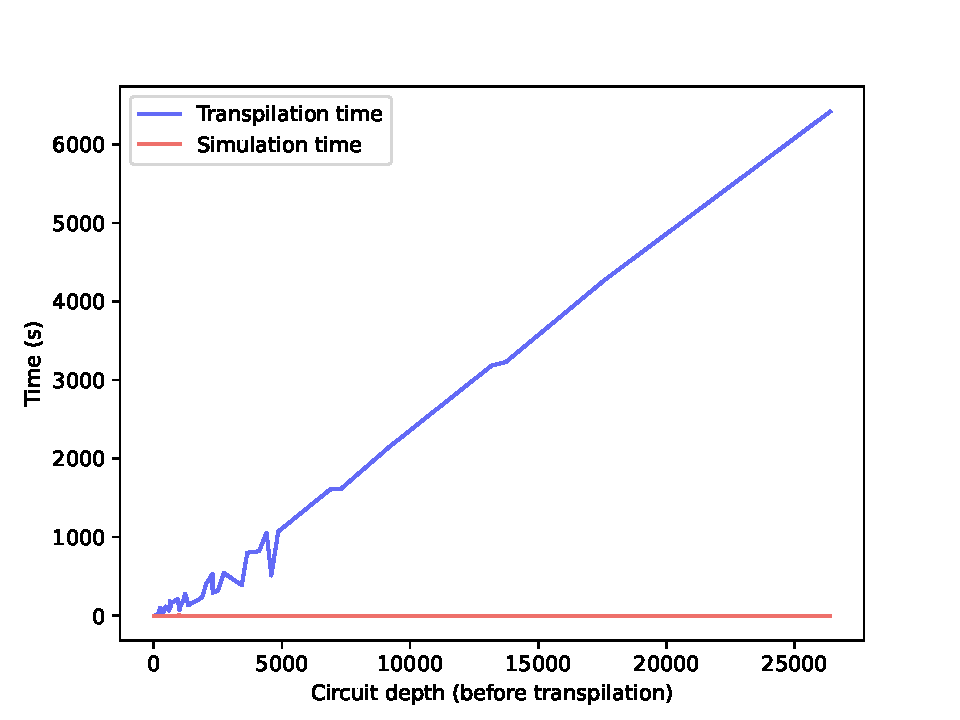
\includegraphics[width=1.1\textwidth]{
          ../src/results/circuit_depth_v_tran_time_and_sim_time-MPS.pdf
      }
      \caption{MPS}
      \label{fig:circuit_depth_v_tran_time_and_sim_time-MPS}
    \end{subfigure}
    \begin{subfigure}{0.48\textwidth}
      \centering
      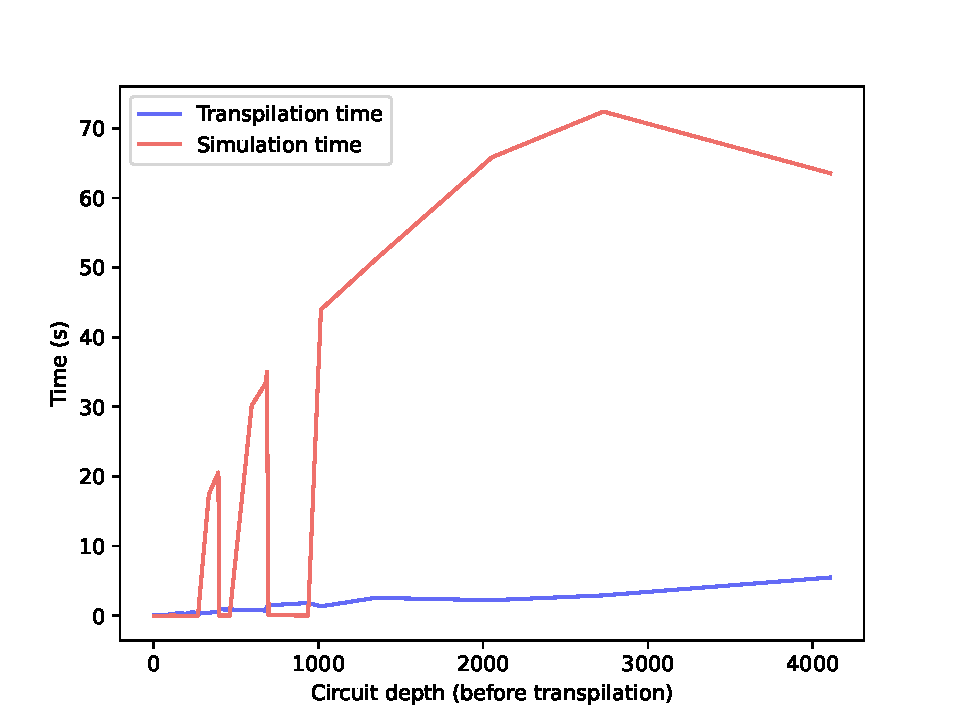
\includegraphics[width=1.1\textwidth]{
          ../src/results/circuit_depth_v_tran_time_and_sim_time-statevector_cpu.pdf
      }
      \caption{Statevector}
      \label{fig:circuit_depth_v_tran_time_and_sim_time-statevector_cpu}
    \end{subfigure}
    \caption{Circuit depth vs Transpilation/Simulation time}
  \end{figure}
\end{frame}


\begin{frame}{Conclusion}
  \begin{itemize}
    \item QVMP can be simulated on moderately-sized inputs, but not large
      enough to observe quantum advantage
    \item Transpilation time and circuit depth can be a bottleneck when scaling to larger circuits
    \item Tooling for automated oracle synthesis is limited
  \end{itemize}
\end{frame}

\begin{frame}{Future work}
  \begin{exampleblock}{Automated synthesis of oracles}
    Extend existing work on reversible compilers to support higher-level
    programming constructs like lists, records, multi-dimensional arrays
  \end{exampleblock}
  \begin{exampleblock}{Better encoding of matrices}
    Investigate more efficient encodings of matrices and related operations
  \end{exampleblock}
  \begin{exampleblock}{Transpilation time bottlenecks}
    Investigate bottle-necks in transpilation
  \end{exampleblock}
\end{frame}

% \begin{frame}[t,fragile]{Future work}
%   \begin{exampleblock}{Automated synthesis of oracles}
%     Extend existing work on reversible compilers to support higher-level
%     programming constructs like lists, records, multi-dimensional arrays
%   \end{exampleblock}
%   \begin{itemize}
%     \item Encoding classical decision functions into quantum circuits is
%       error-prone and cumbersome
%     \item Previous work (REVS, Quipper) have shown that we can automate
%       classical to reversible compilation
%   \end{itemize}
%   \begin{lstlisting}[frame=single,language=ML, numbers=left]
% (* Example program describing the QVMP oracle *)
% 
% [@@oracle]
% let find_row_mismatch a y z =
%   find_idx (fun idx value -> value <> z[idx]) (a * y)
%   \end{lstlisting}
% \end{frame}
% 
% \begin{frame}[t]{Future work (contd)}
%   \begin{exampleblock}{Better encoding of matrices}
%     Investigate more efficient encodings of matrices and related operations
%   \end{exampleblock}
% 
%   \begin{itemize}
%     \item $n$-qubit quantum system can encode a total of $2^n$ states
%     \item QROM is still linear in space complexity
%     \item Alternative approach encodes the entries of the matrix as amplitudes
%       of the quantum system but is harder to work with
%   \end{itemize}
% \end{frame}
% 
% \begin{frame}[t]{Future work (contd)}
%   \begin{exampleblock}{Transpilation time bottlenecks}
%     Investigate bottle-necks in transpilation
%   \end{exampleblock}
%   \begin{itemize}
%     \item Transpilation becomes exponentially slow as the number of qubits
%       increases
%     \item Makes it harder to scale and test circuit implementations
%     \item Cursory investigation into Qiskit's transpile method revealed that
%       SWAPs may be the bottleneck
%   \end{itemize}
% \end{frame}

\begin{frame}{End of talk}
  \begin{centering}
    Questions?
  \end{centering}
\end{frame}

\end{document}
